% Paper for Learning-Based Controls (ME 537)

\documentclass[letterpaper, 10 pt, conference]{ieeeconf}  % Comment this line out if you need a4paper

\IEEEoverridecommandlockouts                              % This command is only needed if 
                                                          % you want to use the \thanks command

\overrideIEEEmargins                                      % Needed to meet printer requirements.

\usepackage{prg-stuff}

\usepackage{caption}
\usepackage{subcaption}
\usepackage{algorithm}
\usepackage[noend]{algpseudocode}

\makeatletter
\def\BState{\State\hskip-\ALG@thistlm}
\makeatother

%\usepackage{ijcai09}  % style
\usepackage{times}    % font
\usepackage{graphicx} % inserting images
\usepackage{cite}
\usepackage{amsmath}
\usepackage{mathtools} % For math
\usepackage{hyperref}
\usepackage{float}
%\usepackage{enumitem}
\renewcommand{\deg}{\ensuremath{^{\circ}}\xspace}  % why doesn't this work???
\captionsetup{justification=centering}

\providecommand{\e}[1]{\ensuremath{\times 10^{#1}}}

\graphicspath{ {./figures/} } % Point to the figures directory

%%%%%%%%%%%%%%%%%%%%%%%%%%%%%%%%%%%%%%%%%%%%%%%%%%%%%%%%%%%%%%%%%%%%%%%%%%%

\title{\LARGE \bf 
Active Planning for Defect Detection in the Knife Domain
}

\author{Austin Nicolai, Kory Kraft, and Gabriel Hackebeil}

\begin{document}

\maketitle
\thispagestyle{empty}
\pagestyle{empty}

\begin{abstract}
\textit{Abstract text will go here}
\let\thefootnote\relax\footnote{\hrulefill
\\\hspace*{1em} \hfill
\\\hspace*{1em} Austin Nicolai and Kory Kraft
\\\hspace*{1em} Robotics Program, School of Mechanical, Industrial, and Manufacturing
\\\hspace*{1em} Engineering, Oregon State University, Corvallis, OR 97331, email: 
\\\hspace*{1em} {\tt\small \{nicolaia, kraftko\}@onid.oregonstate.edu}
\\\hspace*{1em} \hfill
\\\hspace*{1em} Gabriel Hackebeil
\\\hspace*{1em} Computer Science Department, School of Electrical Engineering and
\\\hspace*{1em} Computer Science, Oregon State University, Corvallis, OR 97331, email: 
\\\hspace*{1em} {\tt\small hackebeg@onid.oregonstate.edu}
}
\end{abstract}


\section{Introduction}

Even though automated manufacturing processes can be more consistent than human laborers, defects can occur due to a number of complex internal or external factors. These defects can range from slight cosmetic blemishes to safety-threatening faults \cite{matScience}. The ability to quickly and accurately identify defects as soon as possible within the manufacturing process is important to ensure smooth operation, resource efficiency, and quality products. 

Despite the advanced automated techniques used to manufacture complex products, many products still undergo a manual visual inspection. Yet, the inspection of products is a necessary component of quality control and assurance; using skilled workers for the inspection process however, drains valuable workers away from other important tasks.

With this in mind, we examine automating the defect detection process in the consumer-grade knife domain. The contributions of this paper are twofold:\\

\begin{enumerate}
	\item[1.] We analyze the effectiveness of using computer vision techniques with adaptive planning for active classification.\\
	\item[2.] We successfully apply and test our approach to active classification in the consumer knife domain with real-world data.\\
\end{enumerate}

\section{Related Work}

\subsection{Defect Detection}
Defect detection is key to ensure both quality and safety. The process of manually inspecting parts is tedious and error prone \cite{automatedVisionInspection}. Furthermore, it can be highly mentally and ergonomically repetitive, decreasing employee satisfaction and leading to increased physical strain \cite{evans2005management}\cite{eklund1997ergonomics}. Due to resource constraints within companies, it can sap skilled workers away from productive tasks, leading to economic losses.


Attempts and successes have been made in automating defect detection, but each defect detection process can be highly dependent upon the good manufactured \cite{automatedVisionInspection}\cite{defectGabor}\cite{defectSewer}.

We have decided to focus on defects created during knife manufacturing. One example of this process involves quality control workers visually inspecting batches of knives for a wide variety of defects. Characterization of a defect varies between knife type, defect type, and defect severity. On average, a worker may spend four seconds (two per side) inspecting each knife and typically achieves an accuracy upper-bounded by 80\%.

Our setup is built around this example. We show that active classification for defects in knives is possible using a modern vision sytem united with an adaptive planning algorithm.

\subsection{Computer Vision}

Computer vision, the automated extraction of meaningful information from images, relies on two key components for success: feature extraction and image classification. 

Feature extraction is necessary to deal with the extremely large datasets that comprise a single image; it allows one to cut down the number of features examined from all possible features to a smaller, transformed subset of features that yields the most pertinent information. Feature extraction is different from feature selection in that feature selection simply grabs some subset of the original features and utilizes those \cite{featSelExt}.

While there are general methods currently in use across machine learning to deal with feature extraction (e.g. Principal Component Analysis) and selection, there are specific methods used in computer vision that take advantage of the image data structure.

Image classification is done using common machine learning techniques for classification. Machine learning comes in two forms: supervised and unsupervised. Unsupervised image classification is done by feeding an algorithm a large data set of images or videos and then allowing the machine to pick out the important features and classify these images. While still in its infancy, deep learning with neural networks has been used successfully. The problem with these algorithms at this stage is that they rely on extremely large data sets, can take a long time to train and run, and are not yet ready for a real-time vision system \cite{deepLearning1}. 

Unsupervised learning with image classification requires an expert to label a set of images beforehand. The labeled images are then used to instruct or train the classifier. While more tedious, given a large enough training set, these algorithms can be very efficient and effective.

For example, a real-time vision system for surface defect detection in steel manufacturing was successfully implemented by Jia, et al using standard supervised learning algorithms and a clever feature extraction scheme \cite{steelDefect}. The authors used a rough filter to detect possible edges in the steel and then features are extracted from that according to their pixel length, the gray scale constract of seam to adjacent area, the intensity differences between the two sides of the seams, and the mean and variance of the seam regions. Using these features, the images were then classified using two standard classification algorithms: K-Nearest Neighbors (KNN) and a Support Vector Machine (SVM). The authors were able to classify the images with greater than 90 percent accuracy at a rate of 172 images per second, fast enough to detect defects in real-time for a steel rolling machine that could reach speeds of 225 MPH.

A wavelet filter, Gabor filter, and Gabor wavlet filter were successfully used to classify corrugation defects on rail tracks\cite{railDefect}. In particular, the authors found the Gabor filter to be most successful. The image was first convolved with the Gabor filter at four different orientations. Each of these images were then evaluated with an energy distribution function yielding the mean and variance.  The mean and variance from each filter orientation were assembled to create a feature vector of size 8 for the original image. This is the filter we will be adapting for our approach.

\subsection{Adaptive View Planning}

Informative Path Planning (IPP) is defined as autonomously deciding what path to take while collecting measurements, based on a probabilistic model of the quantity being studied \cite{BNBIPP}. IPP has been effectively used to monitor environmental conditions with autonomous underwater vehicles\cite{BNBIPP}\cite{underwaterIPP}. IPP algorithms, when used in domains that exhibit the property of submodularity (e.g. sensor placement), yield simple greedy solutions that carry the important theoretical guarantee of a close approximation to the optimal solution (within ~63\% of optimal). Additionally, it can be seen that in many cases, greedy solutions are able to perform within 1\% of optimal. 

Adaptive View Planning (AVP) is a specialized case of IPP. AVP seeks to optimize the classification success rate in the shortest amount of time or lowest path cost by having an autonomous agent decide which view angles give the most pertinent information necessary to correctly classify a specific object. The planning is adaptive in the sense that what is seen from one view angle impacts which view angle the agent decide to move to and look at next\cite{hollinger2011active}. 

AVP has been examined in the domain of examining ship hulls for mines \cite{hollinger2011active}. The authors reduced the number of needed views by 80 percent compared to non-adaptive methods.

The detection of defects in knives maps well to the AVP method. A worker might catch a glimmer of light reflecting off the surface of a knife that alerts them to a suspicious area. The worker will then turn the knive in such a way as to clarify whether or not the glimmer was indeed caused by a defect. 

Due to this close mapping and the success of similar methods in other domains, we will be using an adaptive view planning algorithm that utilizes a greedy horizon approach to actively classify one type of defect in a consumer-grade knife.

\section{Methods}

In practice, solving the problem of knife defect detection requires an end-to-end system comprised of a vision system, a knife manipulation system, and an accurate classification system. We focused on implementing a robust vision system and accurate classification system while simulating the knife manipulation system. We use the 4 seconds average as mentioned earlier (S II A) as the time limit that each knife may use before a final assessment as to whether or not it contains a defect.

In particular, we examine a knife with a ding??

\subsection{Data Generation}


A large, comprehensive data set is needed to train a robust classifier capable of accurately detecting surface defects in knives.

To generate our data, the knives were first filmed under a variety of lighting conditions from multiple angles. Still images were then extracted to create a training set. The images selected represent many different angles and several lighting conditions. The image set contains both positive and negative examples of the defect.

Next, a sliding window technique was used to generate additional training data from the image set. This process is shown in \textit{Figure \ref{fig:data generation}}. This was accomplished using a custom program that allows a user to specify the location of all defect corners. From this, the sliding window is able to automatically determine if the region contains a defect. Using this information, the program is able to automatically label the training set data for use in supervised learning.

\begin{figure*}
    \centering
    \begin{subfigure}[b]{.32\textwidth}
        \centering
        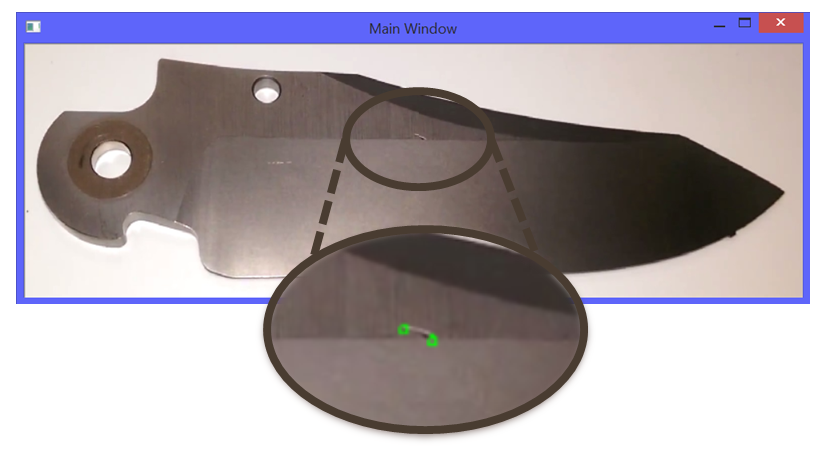
\includegraphics[width=.9\textwidth]{defect_location.png}
        \caption{Selected defect corners}
        \vspace*{2mm}
        \label{fig:defect corners}
    \end{subfigure}
    \hfill
    \begin{subfigure}[b]{.32\textwidth}
        \centering
        \raisebox{8.2mm}
        {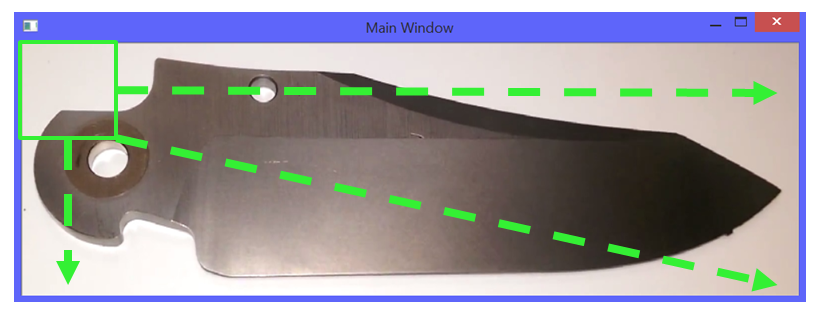
\includegraphics[width=.9\textwidth]{defect_sliding_window.png}}
        \caption{Sliding window}
        \vspace*{2mm}
        \label{fig:sliding window}
    \end{subfigure}
    \hfill
    \begin{subfigure}[b]{.32\textwidth}
        \centering
        \raisebox{1.7mm}
        {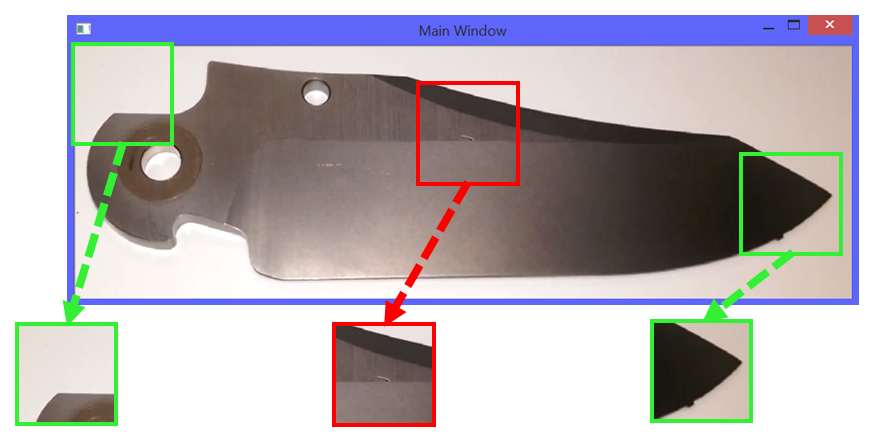
\includegraphics[width=.9\textwidth]{defect_windows.png}}
        \caption{Example labeled windows}
        \vspace*{2mm}
        \label{fig:labeled windows}
    \end{subfigure}
    \caption{Training data generation}
    \label{fig:data generation}
\end{figure*}

\subsection{Computer Vision Algorithm}

The computer vision algorithm employed in this paper was first proposed for use in defect detection in railroad tracks \cite{railDefect}. The algorithm uses Gabor filters and an energy distribution function to extract features from an input image. The classification is performed by an SVM classifier. A flowchart of the algorithm can be seen in \textit{Figure \ref{fig:vision algorithm diagram}}.

First, the input image is fed through a filter bank consisting of Gabor filters. Four wavelet orientations are used: \textit{0\degree}, \textit{45\degree}, \textit{90\degree}, and \textit{135\degree}. Each orientation is replicated for three different filter sizes. This yields a total of twelve filters. Next, the magnitude operator is applied to the filtered images. 

The next step is feature extraction for input into the SVM. The features used are the mean and variance of each filtered image. This allows for an image of high resolution to be collapsed down into a manageable feature set. The final resulting feature vector consists of all means and variances. For our algorithm, the feature vector is of length 24. An example of the entire process can be seen in \textit{Figure \ref{fig:gabor filter bank}}.

\begin{figure*}
    \centering
    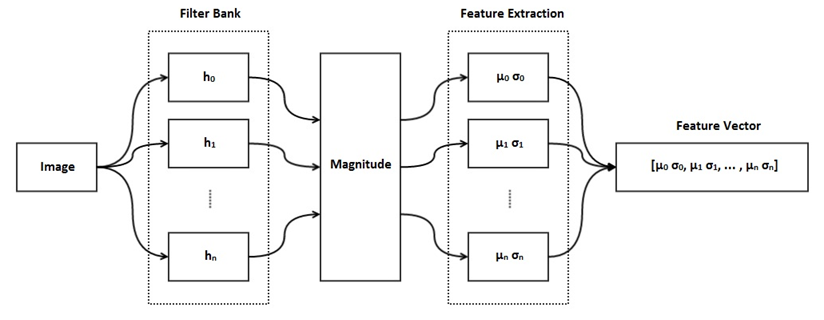
\includegraphics[width=.75\textwidth]{computer_vision_diagram.png}
    \caption{Computer vision algorithm flowchart}
    \vspace*{2mm}
    \label{fig:vision algorithm diagram}
\end{figure*}

\begin{figure}
    \centering
    \begin{subfigure}[b]{.49\textwidth}
        \centering
        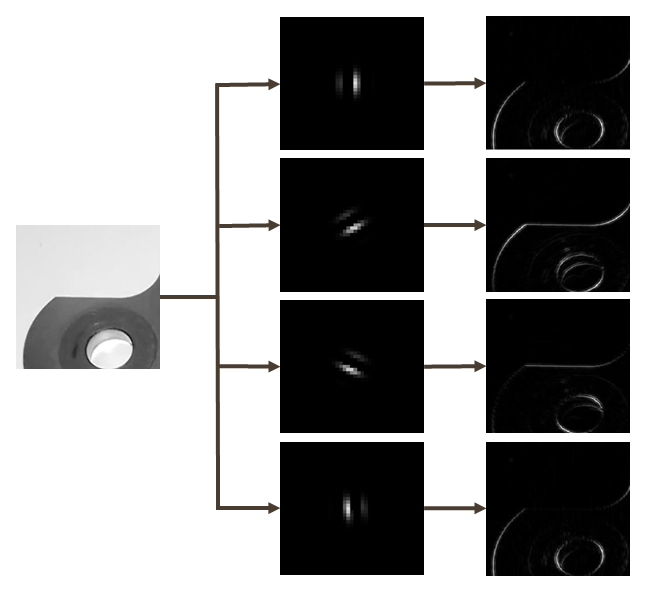
\includegraphics[width=.65\textwidth]{gabor_filter_small.png}
        \caption{Small Gabor filter bank}
        \vspace*{2mm}
        \label{fig:small gabor}
    \end{subfigure}
    \hfill
    \begin{subfigure}[b]{.49\textwidth}
        \centering
        {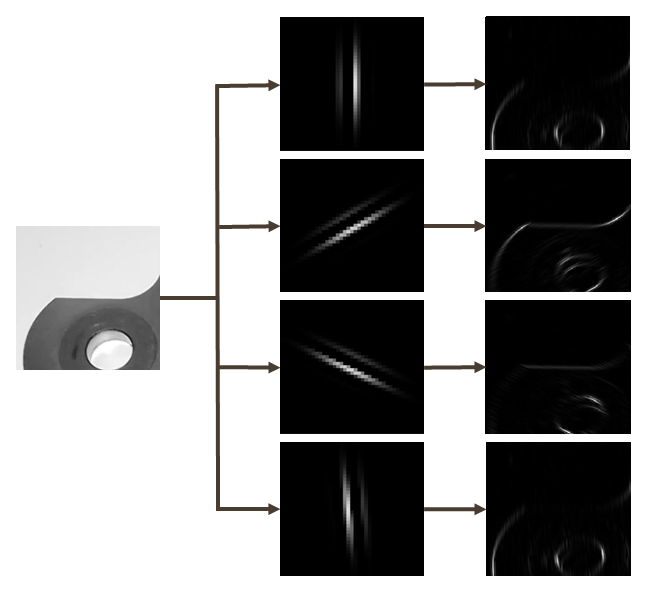
\includegraphics[width=.65\textwidth]{gabor_filter_large.png}}
        \caption{Large Gabor filter bank}
        \vspace*{2mm}
        \label{fig:large gabor}
    \end{subfigure}
    \caption{Gabor filter bank examples}
    \label{fig:gabor filter bank}
\end{figure}

\subsection{Adaptive Planning}

Given the output of the vision system, we actively classify the knife as containing a defect or not by using a greedy horizon planner to reduce the entropy of the belief of all the regions of the knife. We simulate the robotic manipulation of the knife by characterizing each view angle as a state. The planner then decides, given a current state, which state to view next based on what has been seen up to the given point. A movement cost is incurred from one view state to another using the angular Manhattan distance as a metric. This assumes that the camera is situated perpendicular to the knife in the x and y axes initially. Additionally, a simulated "camera view time" is added to the movement cost. This view time simulates the time requires to take and process a single image.

We start with an initial belief that the knife has a defect in each region at 50\%.

\begin{equation*}
    P(D_i)^{\theta_0} = 0.5 \label{eq: initDist}
\end{equation*}

Based on the experimental runs, we characterize the vision system as 80\% accurate.

\begin{equation*}
    P(\mathbf{e}|D_i) \in \{0.2,0.8\} \label{eq:initVisionAccuracy}
\end{equation*}

To make an accurate classification of the knife, the total entropy for all knife regions is minimized. This, in turn, increases the confidence about our belief for a given knife region. The total entropy of the knife is formulated in terms of individual knife regions as:

\begin{equation}
    % \begin{equation}
    H(\theta) = \sum_{i\in\mathcal{K}} H(P(D_i)^\theta) \label{eq: totalKnifeEntropyDist}
\end{equation}


After selecting a view (whether randomly or using the greedy horizon planner), a Bayesian update is performed over all the knife regions based on what is predicted at the current view.

\begin{equation}
    P(D_i|\mathbf{e}) = \frac{P(\mathbf{e}|D_i) P(D_i)}{P(\mathbf{e})}, \;\;i\in \mathcal{K}  \label{eq: bayesianUpdate}
\end{equation}

The value in selecting the next view is captured by the Bayesian update. When available, historical data can be used to predict in which knife regions defects can be reliably seen, thereby effecting the value of $P(\mathbf{e}|D_i)$. In the absence of such data, one might consider placing a level of confidence on the performance of the image classification system over a knife region given a certain view angle. Such an update might take the form of Equation \eqref{confidenceValueUpdate} below.

\begin{equation}
    P(D_i)^{\theta_{t+1}} = \beta_i^{\theta} P(D_i|\mathbf{e}) + (1 - \beta_i^{\theta}) P(D_i)^{t} \label{confidenceValueUpdate}
\end{equation}

For this study we simulate a form of perspective correction and assign confidences $\beta_i^{\theta} \in [0.3 - 0.85], \;\;i\in\mathcal{K},\;\theta\in\Theta^t$, where larger confidence values are assigned based on what can feasibly and reliably be seen from a given view angle. Given these predictions to how a new view angle will update the knife region probabilities, we assign a value to moving to the next view as

\begin{equation}
    \text{MoveValue}(\theta_{t+1}) = \frac{H(\theta_t) - H(\theta_{t+1})}{\text{MoveCost}(\theta_t,\theta_{t+1})}. \label{entropyReduction}
\end{equation}

 This equation balances the predicted information gained from the considered next view with the budget cost of moving to this view. Thus for the single lookahead greedy search, the next view is chosen by maximizing Equation \eqref{entropyReduction}.

\begin{equation}
    \theta_{t+1} = \underset{\theta'\in\Theta^t}{\text{argmax}}\text{ MoveValue}(\theta')
\end{equation}

\begin{figure*}
    \centering
    \begin{subfigure}[b]{.24\textwidth}
        \centering
        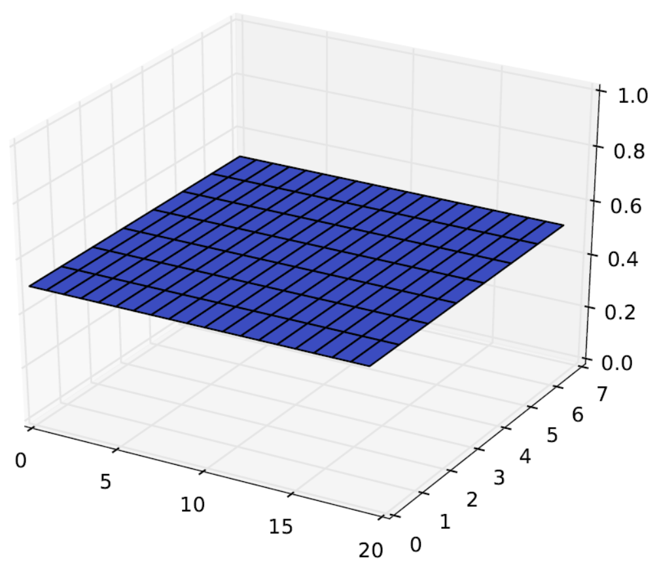
\includegraphics[width=.99\textwidth]{greedy1.png}
        \caption{Greedy selection \\ after 0 views}
        \vspace*{2mm}
        \label{fig:greedy0view}
    \end{subfigure}
    \hfill
    \begin{subfigure}[b]{.24\textwidth}
        \centering
        {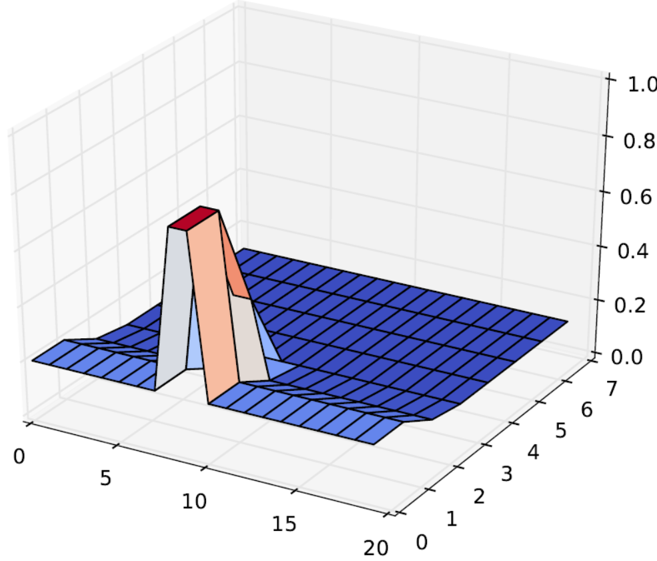
\includegraphics[width=.99\textwidth]{greedy2.png}}
        \caption{Greedy selection \\ after 2 views}
        \vspace*{2mm}
        \label{fig:greedy2view}
    \end{subfigure}
    \hfill
    \begin{subfigure}[b]{.24\textwidth}
        \centering
        {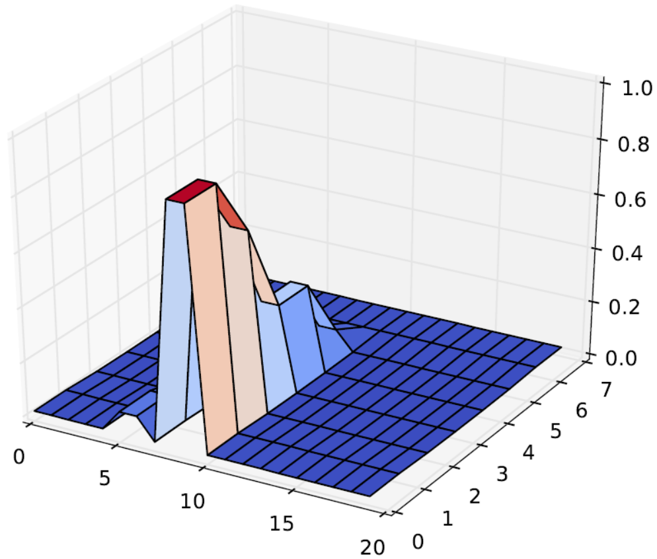
\includegraphics[width=.99\textwidth]{greedy3.png}}
        \caption{Greedy selection \\ after 5 views}
        \vspace*{2mm}
        \label{fig:greedy5view}
    \end{subfigure}
    \hfill
    \begin{subfigure}[b]{.24\textwidth}
        \centering
        {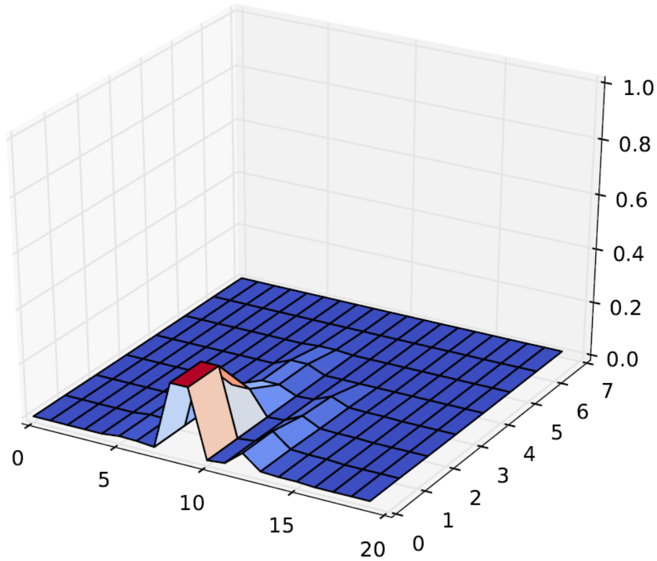
\includegraphics[width=.99\textwidth]{greedy4.png}}
        \caption{Greedy selection \\ after 8 views}
        \vspace*{2mm}
        \label{fig:greedy8view}
    \end{subfigure}
    \hfill
    \begin{subfigure}[b]{.24\textwidth}
        \centering
        {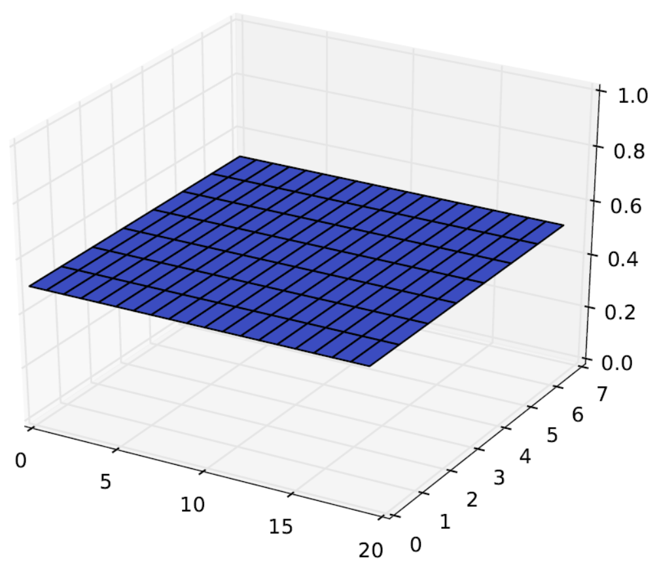
\includegraphics[width=.99\textwidth]{random1.png}}
        \caption{Random selection \\ after 0 views}
        \vspace*{2mm}
        \label{fig:rand0view}
    \end{subfigure}
    \hfill
    \begin{subfigure}[b]{.24\textwidth}
        \centering
        {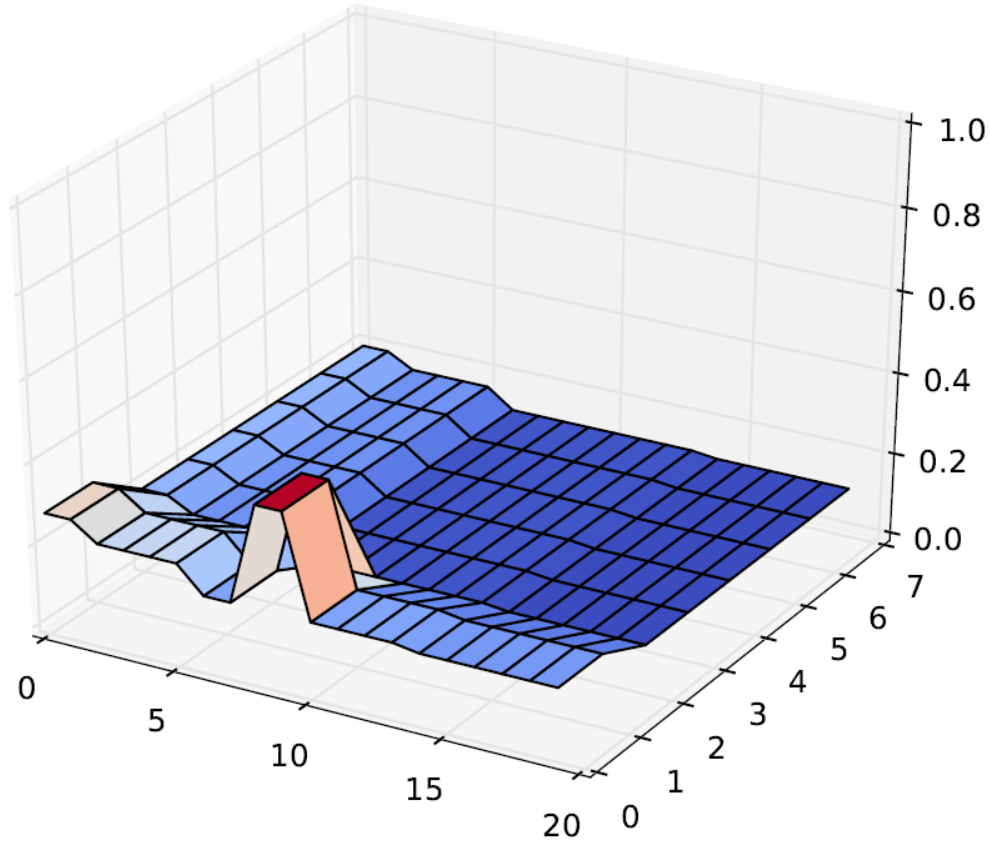
\includegraphics[width=.99\textwidth]{random2.png}}
        \caption{Random selection \\ after 2 views}
        \vspace*{2mm}
        \label{fig:rand2view}
    \end{subfigure}
    \hfill
    \begin{subfigure}[b]{.24\textwidth}
        \centering
        {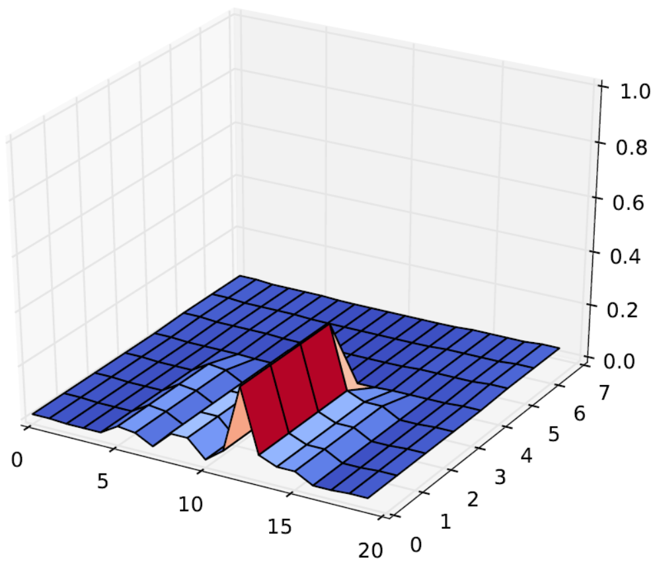
\includegraphics[width=.99\textwidth]{random3.png}}
        \caption{Random selection \\ after 5 views}
        \vspace*{2mm}
        \label{fig:rand5view}
    \end{subfigure}
    \hfill
    \begin{subfigure}[b]{.24\textwidth}
        \centering
        {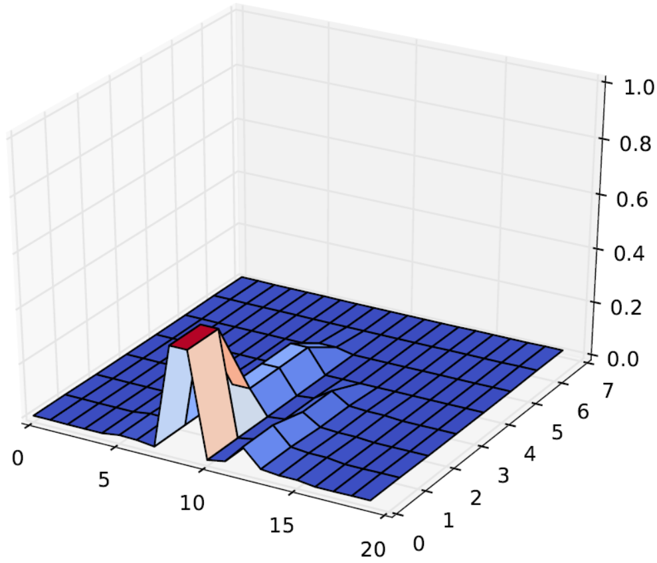
\includegraphics[width=.99\textwidth]{random4.png}}
        \caption{Random selection \\ after 7 views}
        \vspace*{2mm}
        \label{fig:rand7view}
    \end{subfigure}
    \caption{Probability of defect by knife region. Note that the greedy \\ selection achieves 8 views in the time budget while the random \\ selection only achieves 7 views in the same time frame.}
    \label{fig:prob_dists}
\end{figure*}

\begin{figure}
    \centering
    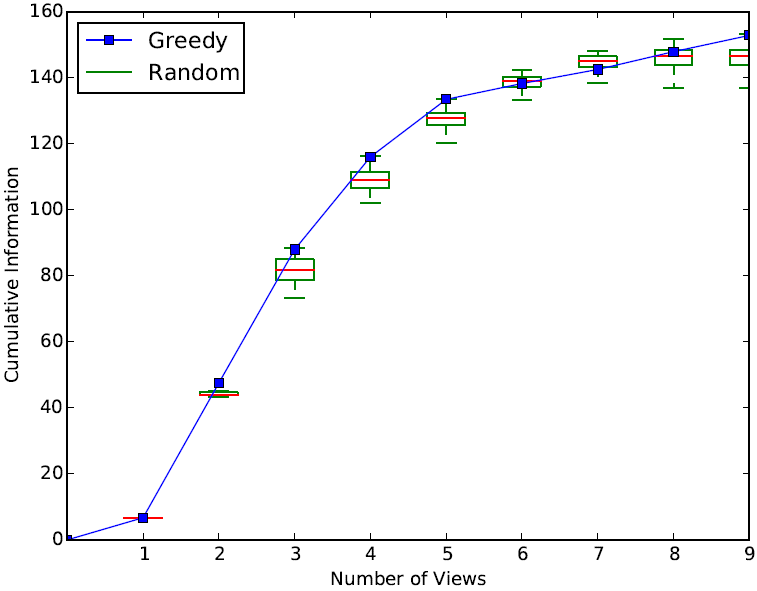
\includegraphics[width=.49\textwidth]{info_gain_views.png}
    \caption{Cumulative information gained}
    \vspace*{2mm}
    \label{fig:cumulative_info}
\end{figure}

\section{Results}

\subsection{Computer Vision Algorithm}

Initial testing of the proposed vision algorithm shows good results. Initial results show that for training, validation, and test data sets, the defect detection rate is greater than 80\%. It is important to note that while promising, these results were generated from a limited data set in terms of knife and defect examples. Increasing the number of examples, both positive and negative, in the data set will yield a more robust classifier.

While additional parameter tuning in the vision algorithm may yield higher detection rate, there are other avenues to explore. These avenues include the use of alternative lighting sources (e.g. near field, dark field), as previously mentioned. The use of these lighting sources may help to increase the visibility of defects, and thus make them easier to classify. This, in turn, will lead to a higher defect detection rate for the classifier.

\subsection{Planning Algorithm}

\section{Discussion}

\textit{Discussion text will go here}

\section{Conclusions and Future Work}

In this paper, we show that current computer vision techniques are successful in classifying a single surface defect on a knife. Additionally, we show that using these vision techniques in conjunction with real world data allows a simple greedy adaptive planner to outperform random view selection. While the results in this paper are promising, there are two main avenues for future work.

First, there is room to explore more sophisticated planning methods. These include planning with a longer horizon as well as planning over a larger number of views. Since the current algorithm processes so quickly, planning with a longer horizon would allow for the algorithm to maximize the long term information gain. As new information from the vision system is received, the plan can be updated. Additionally, it would be interesting to see the effects of a larger set of possible view angles. Specifically, using views with rotations along multiple axes may provide interesting results.

Second, the nature of the task begs the question of if the view planning algorithm can be improved by incorporating inspection data from human operators. The motivation behind this is that through experience, skilled human inspectors build a large knowledge base of how/where defects typically present. This allows them to inspect knives more effectively than a novice. We theorize that in most cases, human inspectors will follow a general view sequence that they have learned works well. When the inspector notices something that is a potential defect, they may adjust their inspection sequence to more closely inspect that area. This data can be incorporated into the adaptive planning algorithm by using it to help predict the information gains of the set of possible next views. That is, based on the results of the vision system and human inspection data, we may be able to boost (or reduce) the predicted information gain of certain views.

\bibliographystyle{IEEEtran}
\bibliography{main}


\end{document}

% FIGURE HINTS 
%
%\begin{figure*}
%    \centering
%    \begin{subfigure}[b]{0.3\textwidth}
%        \centering
%        \includegraphics[width=.7\textwidth]{Reflex.jpg}
%        \caption{Reflex agent path}
%        \label{fig:reflex path}
%    \end{subfigure}
%    \hfill
%    \begin{subfigure}[b]{0.3\textwidth}
%        \centering
%        \includegraphics[width=.7\textwidth]{Random.jpg}
%        \caption{Random agent path}
%        \label{fig:random path}
%    \end{subfigure}
%    \hfill
%    \begin{subfigure}[b]{0.3\textwidth}
%        \centering
%        \includegraphics[width=.7\textwidth]{Memory.jpg}
%        \caption{Memory agent path}
%        \label{fig:memory path}
%    \end{subfigure}
%    \caption{Agent paths}
%    \label{fig:agent paths}
%\end{figure*}

% ALGORITHM HINTS
%
%\begin{algorithm}[h]
%\caption{Reflex agent}\label{reflex algorithm}
%\begin{algorithmic}[1]
%\If {$isDirty = true$}
%\State \Return \textit{actionSuck}
%\ElsIf {$facingWall \neq true$}
%\State \Return \textit{actionForward}
%\ElsIf {$facingWall = true$ AND $isHome = true$}
%\State \Return \textit{actionOff}
%\Else
%\State \Return \textit{actionTurnRight}
%\EndIf
%\end{algorithmic}
%\end{algorithm}
